\hypertarget{ch:llnclt}{%
\chapter{The Law of Large Numbers and the Central Limit Theorem}\label{ch:llnclt}}

\section{Introduction}
Let's start with a couple of simple examples:
\begin{enumerate}
\item We get a random sample of 200 people and give them an IQ test. What is the distribution of the scores in this sample? How close is it to the true distribution of the whole population?\\
How likely is it that we find a person with IQ greater than 150?\\
In order to be accepted to the Mensa club a person has to be in the top 2\% of the IQ distribution. What is the minimum score required in order to be a Mensa member?
\item The pockets of the roulette wheel are numbered from 0 to 36. In number ranges from 1 to 10 and 19 to 28, odd numbers are red and even are black. In ranges from 11 to 18 and 29 to 36, odd numbers are black and even are red. There is a green pocket numbered 0 (zero). Suppose you want to bet on a color, say, red, and if the ball lands in a red pocket your payoff is twice your bet, and otherwise you lose your bet. What is the probability you win? What is your expected payoff? Suppose you have \$10,000, and you bet one dollar each time. How much money will you win or lose?.
\item Suppose that you get a text message every 6 minutes (a rate of 10 per hour), and suppose that they arrive independently of one another, according to a Poisson distribution. How many messages do you expect to get on an average day, between 8am and 8pm? 
\item \hb{homework question?}As of June 16, 2021 Tony Snell from the Atlanta Hawks leads the NBA in 3pt accuracy with 53.8\%.
If he takes 3pt 10 shots per game over the next 10 games, how many three-point shots do you expect him to make?
\item \hb{homework question?}In 2021 the boy to girl birth ratio in the USA is estimated to be 1.05. If we took a random sample of 300 newborns across the USA, how many do you expect to be boys?
\end{enumerate}

The main paradigm in statistical inference and prediction in order to answer such question is to take a sample from the population we're interested in, and choose a mathematical model which we believe represents the whole population. Then we check if our model appears to reasonable, in the sense that it fits the data well. If it does, we can use the mathematical properties of the model to draw conclusions about the population. By representing the sample using a mathematical (probabilistic) formula, we essentially augment a finite sample to an infinite one. Working with a formula/model for the data allows us to use the `heavy artillery' of math, like finding maximum/minimum, computing areas under the curve of the function, and so on. 

This chapter deals with inference which can be derived from the mean of a population, and we show the (arguably) two most important results in statistics -- the law of large numbers (LLN), and the central limit theorem (CLT). Together, these two very general theorems make it possible to draw conclusions about the whole population, from a single sample! (as long as the sample size is large enough).


\section{The Law of Large Numbers}

\subsection{Example \#1 -- the IQ score}
We get a random sample of 200 people and give them an IQ test. From this sample, we want to infer the true distribution in the entire population.

Suppose that the IQ in the general population has a normal distribution with mean=100 and  standard deviation =15, and from this population we draw 200 people, and calculate the sample mean and standard deviation:

\begin{knitrout}
\definecolor{shadecolor}{rgb}{0.969, 0.969, 0.969}\color{fgcolor}\begin{kframe}
\begin{alltt}
\hlkwd{set.seed}\hlstd{(}\hlnum{95473}\hlstd{)}
\hlstd{n} \hlkwb{<-} \hlnum{200}
\hlstd{samp} \hlkwb{<-} \hlkwd{rnorm}\hlstd{(n,} \hlnum{100}\hlstd{,} \hlnum{15}\hlstd{)}
\hlkwd{cat}\hlstd{(}\hlstr{"Mean="}\hlstd{,}\hlkwd{mean}\hlstd{(samp),} \hlstr{", SD="}\hlstd{,}\hlkwd{sd}\hlstd{(samp),}\hlstr{"\textbackslash{}n"}\hlstd{)}
\end{alltt}
\begin{verbatim}
## Mean= 99.38613 , SD= 15.55667
\end{verbatim}
\end{kframe}
\end{knitrout}

We notice that the sample mean is 99.4 and the sample standard deviation is 15.6. Both are very close to the true values. 

Let's pretend that just like in real life, we don't know the true distribution, so we have to check if the mathematical model we chose (normal distribution) is appropriate for the data from the finite sample. When it is assumed that the data come from a normal distribution, we can use the \code{qqnorm} function to check if the assumption is reasonable:

\begin{knitrout}
\definecolor{shadecolor}{rgb}{0.969, 0.969, 0.969}\color{fgcolor}\begin{kframe}
\begin{alltt}
\hlkwd{qqnorm}\hlstd{(samp,} \hlkwc{cex}\hlstd{=}\hlnum{0.7}\hlstd{,} \hlkwc{pch}\hlstd{=}\hlnum{18}\hlstd{,} \hlkwc{col}\hlstd{=}\hlstr{"purple"}\hlstd{)}
\hlkwd{abline}\hlstd{(}\hlnum{100}\hlstd{,}\hlnum{15}\hlstd{,}\hlkwc{col}\hlstd{=}\hlstr{"orange"}\hlstd{,} \hlkwc{lwd}\hlstd{=}\hlnum{3}\hlstd{)}
\end{alltt}
\end{kframe}\begin{figure}

{\centering 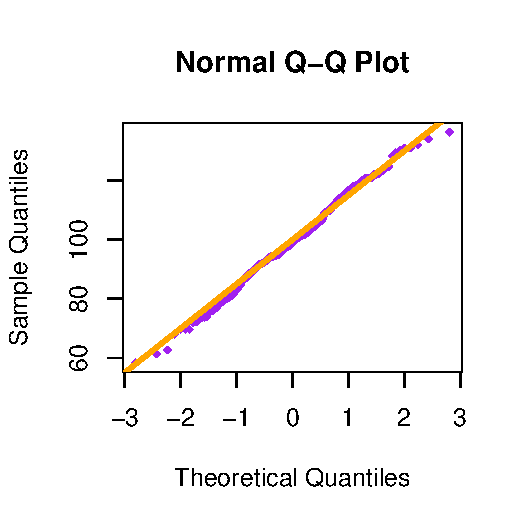
\includegraphics[width=\maxwidth]{figure/intro-lln1-1-1} 

}

\caption[Q-Q plot for the simulated IQ scores]{Q-Q plot for the simulated IQ scores.}\label{fig:intro-lln1-1}
\end{figure}

\end{knitrout}

The points in the Q-Q plot lie very close to a straight line, indicating that the sample  was  likely drawn from a normal distribution (because we generated it this way, this is not surprising. However, when we get a random sample and we do not know the true distribution, this plot is useful to check whether our mathematical model is reasonable.)

To understand what the LLN, let's obtain samples of varying sizes and see what happens to the sample mean as we increase $n$. 

\begin{knitrout}
\definecolor{shadecolor}{rgb}{0.969, 0.969, 0.969}\color{fgcolor}\begin{kframe}
\begin{alltt}
\hlkwd{set.seed}\hlstd{(}\hlnum{95473}\hlstd{)}
\hlstd{ns} \hlkwb{<-} \hlkwd{seq}\hlstd{(}\hlnum{10}\hlstd{,} \hlnum{2000}\hlstd{,} \hlkwc{by}\hlstd{=}\hlnum{10}\hlstd{)}
\hlstd{L} \hlkwb{<-} \hlkwd{length}\hlstd{(ns)}
\hlstd{allMeans} \hlkwb{<-} \hlkwd{rep}\hlstd{(}\hlnum{0}\hlstd{, L)}
\hlkwa{for} \hlstd{(i} \hlkwa{in} \hlnum{1}\hlopt{:}\hlstd{L) \{}
  \hlstd{samp} \hlkwb{<-} \hlkwd{rnorm}\hlstd{(ns[i],} \hlnum{100}\hlstd{,} \hlnum{15}\hlstd{)}
  \hlstd{allMeans[i]} \hlkwb{<-} \hlkwd{mean}\hlstd{(samp)}
\hlstd{\}}
\hlkwd{plot}\hlstd{(ns, allMeans,} \hlkwc{pch}\hlstd{=}\hlnum{19}\hlstd{,} \hlkwc{cex}\hlstd{=}\hlnum{0.5}\hlstd{,} \hlkwc{col}\hlstd{=}\hlnum{3}\hlstd{,} \hlkwc{axes}\hlstd{=}\hlnum{FALSE}\hlstd{)}
\hlkwd{axis}\hlstd{(}\hlnum{1}\hlstd{);} \hlkwd{axis}\hlstd{(}\hlnum{2}\hlstd{)}
\hlkwd{abline}\hlstd{(}\hlkwc{h}\hlstd{=}\hlnum{100}\hlstd{,} \hlkwc{lwd}\hlstd{=}\hlnum{3}\hlstd{,}\hlkwc{col}\hlstd{=}\hlnum{2}\hlstd{)}
\end{alltt}
\end{kframe}\begin{figure}

{\centering 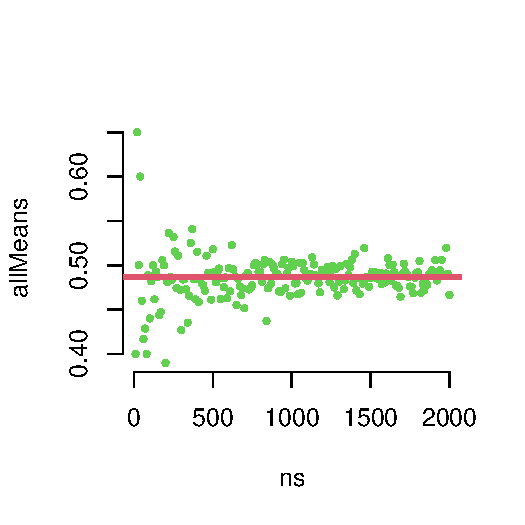
\includegraphics[width=\maxwidth]{figure/intro-lln1-2-1} 

}

\caption[Q-Q plot for the simulated IQ scores]{Q-Q plot for the simulated IQ scores.}\label{fig:intro-lln1-2}
\end{figure}

\end{knitrout}

We see that as $n$ increases, the sample mean gets closer to the true mean (100).



\subsection{Example \#2 -- the roulette wheel}
Here, the outcome is binary -- we either win or lose. The probability of winning if we choose the red color, is $18/37$.
Let's simulate 40 bets at the roulette wheel, where, in each we put a dollar on red. Each bet is won with a Bernoulli distribution, $Ber(18/37)$ and we repeat it 40 times. Equivalently, we can look at it as a single binomial sample, with $n=40$ and $p=18/37$.

\begin{knitrout}
\definecolor{shadecolor}{rgb}{0.969, 0.969, 0.969}\color{fgcolor}\begin{kframe}
\begin{alltt}
\hlkwd{set.seed}\hlstd{(}\hlnum{75473}\hlstd{)}
\hlstd{n} \hlkwb{<-} \hlnum{40}
\hlstd{samp} \hlkwb{<-} \hlkwd{rbinom}\hlstd{(n,} \hlkwc{size}\hlstd{=}\hlnum{1}\hlstd{,} \hlkwc{prob}\hlstd{=}\hlnum{18}\hlopt{/}\hlnum{37}\hlstd{)}
\hlkwd{cat}\hlstd{(}\hlstr{"Mean="}\hlstd{,}\hlkwd{mean}\hlstd{(samp),} \hlstr{", SD="}\hlstd{,}\hlkwd{sd}\hlstd{(samp),}\hlstr{"\textbackslash{}n"}\hlstd{)}
\end{alltt}
\begin{verbatim}
## Mean= 0.575 , SD= 0.5006406
\end{verbatim}
\end{kframe}
\end{knitrout}

Notice that in those 40 bets, our probability of winning was 0.575 (greater than 0.5.) This seems great -- if we keep going we might get rich. However, let's see what happens to the sample mean as we increase $n$. 

\begin{knitrout}
\definecolor{shadecolor}{rgb}{0.969, 0.969, 0.969}\color{fgcolor}\begin{kframe}
\begin{alltt}
\hlkwd{set.seed}\hlstd{(}\hlnum{95473}\hlstd{)}
\hlstd{ns} \hlkwb{<-} \hlkwd{seq}\hlstd{(}\hlnum{10}\hlstd{,} \hlnum{2000}\hlstd{,} \hlkwc{by}\hlstd{=}\hlnum{10}\hlstd{)}
\hlstd{L} \hlkwb{<-} \hlkwd{length}\hlstd{(ns)}
\hlstd{allMeans} \hlkwb{<-} \hlkwd{rep}\hlstd{(}\hlnum{0}\hlstd{, L)}
\hlkwa{for} \hlstd{(i} \hlkwa{in} \hlnum{1}\hlopt{:}\hlstd{L) \{}
  \hlstd{samp} \hlkwb{<-} \hlkwd{rbinom}\hlstd{(ns[i],} \hlkwc{size}\hlstd{=}\hlnum{1}\hlstd{,} \hlkwc{prob}\hlstd{=}\hlnum{18}\hlopt{/}\hlnum{37}\hlstd{)}
  \hlstd{allMeans[i]} \hlkwb{<-} \hlkwd{mean}\hlstd{(samp)}
\hlstd{\}}
\hlkwd{plot}\hlstd{(ns, allMeans,} \hlkwc{pch}\hlstd{=}\hlnum{19}\hlstd{,} \hlkwc{cex}\hlstd{=}\hlnum{0.5}\hlstd{,} \hlkwc{col}\hlstd{=}\hlnum{3}\hlstd{,} \hlkwc{axes}\hlstd{=}\hlnum{FALSE}\hlstd{)}
\hlkwd{axis}\hlstd{(}\hlnum{1}\hlstd{);} \hlkwd{axis}\hlstd{(}\hlnum{2}\hlstd{)}
\hlkwd{abline}\hlstd{(}\hlkwc{h}\hlstd{=}\hlnum{18}\hlopt{/}\hlnum{37}\hlstd{,} \hlkwc{lwd}\hlstd{=}\hlnum{3}\hlstd{,}\hlkwc{col}\hlstd{=}\hlnum{2}\hlstd{)}
\end{alltt}
\end{kframe}\begin{figure}

{\centering 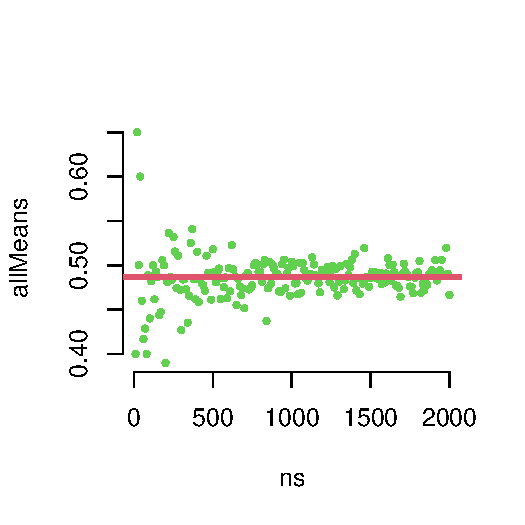
\includegraphics[width=\maxwidth]{figure/intro-lln1-2-1} 

}

\caption[The sample mean from n bets at the roulette wheel]{The sample mean from n bets at the roulette wheel.}\label{fig:intro-lln1-2}
\end{figure}

\end{knitrout}

As before, the sample mean gets closer to the true mean of the distribution, which is $p=18/37$, which is less than 0.5, so if we keep placing bets we will end up losing money. In fact, we can check how much we will lose if we bet \$1 each time, and do it 10,000 time

\begin{knitrout}
\definecolor{shadecolor}{rgb}{0.969, 0.969, 0.969}\color{fgcolor}\begin{kframe}
\begin{alltt}
\hlstd{n} \hlkwb{<-} \hlnum{10000}
\hlstd{roulette} \hlkwb{<-} \hlkwd{rbinom}\hlstd{(n,} \hlnum{1}\hlstd{,} \hlnum{18}\hlopt{/}\hlnum{37}\hlstd{)}
\hlkwd{cat}\hlstd{(}\hlstr{"Prob. win="}\hlstd{,} \hlkwd{mean}\hlstd{(roulette),}\hlstr{"\textbackslash{}n"}\hlstd{)}
\end{alltt}
\begin{verbatim}
## Prob. win= 0.4898
\end{verbatim}
\begin{alltt}
\hlkwd{cat}\hlstd{(}\hlstr{"Paid: $"}\hlstd{,} \hlkwd{prettyNum}\hlstd{(n,} \hlkwc{big.mark}\hlstd{=}\hlstr{","}\hlstd{),} \hlstr{". Won: "}\hlstd{,} \hlkwd{sum}\hlstd{(roulette),} \hlstr{"times."}\hlstd{,} \hlstr{"Total gain:"}\hlstd{,} \hlkwd{prettyNum}\hlstd{(}\hlnum{2}\hlopt{*}\hlkwd{sum}\hlstd{(roulette),} \hlkwc{big.mark} \hlstd{=} \hlstr{","}\hlstd{),} \hlstr{"dollars. Net gain/loss:"}\hlstd{,} \hlkwd{prettyNum}\hlstd{(}\hlnum{2}\hlopt{*}\hlkwd{sum}\hlstd{(roulette)}\hlopt{-}\hlstd{n,}\hlkwc{big.mark} \hlstd{=} \hlstr{","}\hlstd{),}\hlstr{"\textbackslash{}n"}\hlstd{)}
\end{alltt}
\begin{verbatim}
## Paid: $ 10,000 . Won:  4898 times. Total gain: 9,796 dollars. Net gain/loss: -204
\end{verbatim}
\end{kframe}
\end{knitrout}

To the casino it doesn't matter if one person bets \$1,000,000 or if 1,000 people each bets on \$1,000 -- in both cases the casino will win with probability 19/37.


\subsection{Example \#3 -- receiving test messages}
Let's simulate $n$ days, and in each one count the number of messages, if they arrive independently from a Poisson distribution with rate=10. In each day we count messages over 12 hours, so notice that how we multiply by 12 in the code below.

\begin{knitrout}
\definecolor{shadecolor}{rgb}{0.969, 0.969, 0.969}\color{fgcolor}\begin{kframe}
\begin{alltt}
\hlstd{ssize} \hlkwb{<-} \hlkwd{c}\hlstd{(}\hlnum{5}\hlstd{,}\hlkwd{seq}\hlstd{(}\hlnum{10}\hlstd{,}\hlnum{1000}\hlstd{,}\hlkwc{by}\hlstd{=}\hlnum{10}\hlstd{))}
\hlstd{myMsg} \hlkwb{<-} \hlkwd{rep}\hlstd{(}\hlnum{0}\hlstd{,}\hlkwd{length}\hlstd{(ssize))}
\hlkwd{set.seed}\hlstd{((}\hlnum{40001}\hlstd{))}
\hlkwa{for} \hlstd{(i} \hlkwa{in} \hlnum{1}\hlopt{:}\hlkwd{length}\hlstd{(ssize)) \{}
    \hlstd{myMsg[i]} \hlkwb{<-} \hlkwd{mean}\hlstd{(}\hlnum{12}\hlopt{*}\hlkwd{rpois}\hlstd{(ssize[i],} \hlnum{10}\hlstd{))}
\hlstd{\}}
\hlkwd{plot}\hlstd{(ssize, myMsg,}\hlkwc{pch}\hlstd{=}\hlnum{17}\hlstd{,}\hlkwc{col}\hlstd{=}\hlstr{"blue"}\hlstd{,} \hlkwc{axes}\hlstd{=}\hlnum{FALSE}\hlstd{)}
\hlkwd{axis}\hlstd{(}\hlnum{1}\hlstd{);} \hlkwd{axis}\hlstd{(}\hlnum{2}\hlstd{)}
\hlkwd{abline}\hlstd{(}\hlkwc{h}\hlstd{=}\hlnum{12}\hlopt{*}\hlnum{10}\hlstd{,} \hlkwc{lwd}\hlstd{=}\hlnum{2}\hlstd{,}\hlkwc{col}\hlstd{=}\hlnum{2}\hlstd{)}
\end{alltt}
\end{kframe}\begin{figure}

{\centering 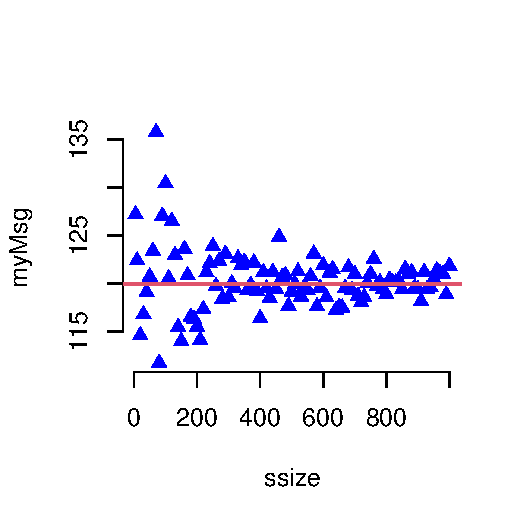
\includegraphics[width=\maxwidth]{figure/intro-lln2-0-1} 

}

\caption[Simulated text messages]{Simulated text messages.}\label{fig:intro-lln2-0}
\end{figure}

\end{knitrout}


If we continue to get text messages at this fixed rate over a long period of time, and we calculate the average daily messages (from 8am to 8pm) we see that that average converges to 12*10=120 messages per day. 


\subsection{The LLN -- an intuitive statement of the theorem}
Informally, the law of large number states that the results of an experiment tend to settle down to a fixed average when the experiment is repeated many times. In other words, as the sample size increases, the sample mean will get closer to the true population mean.

The LLN is very general -- it doesn't matter if the question is about how many boy-births we expect to see (`binomial distribution') or if we measure IQ (`normal distribution'). The only requirements are that the samples are independent, and identically distributed, and that the true distribution actually has a mean. (We will see an example where this is not the case.)

It is important to emphasize that the LLN does not imply that the results of future experiments will balance out what already happened! If we bet 100 times at the roulette wheel and lost each time, this does not mean that we have a better chance of winning the next bet. All the LLN is saying is that if we continue to play many times, the overall probability that we win in each round will converge to 18/37.

\subsection{Example \#4 -- when the LLN doesn't work}
We have two groups of students who have to take a math test. Group A has a mean score of 70 and a standard deviation of 10, while group B has mean 60 and standard deviation 20. Both groups have a normal distribution.
We take a sample of size $n$ from each group and calculate the sample means. Then, we calculate the difference between the sample means, $d_{AB}=\bar{x}_A-\bar{x}_B$, and the ratio between the means, $r_{AB}=\bar{x}_A/\bar{x}_B$.
As before, we increase the sample size and see how it affects $d_{AB}$ and $r_{AB}$.

\begin{knitrout}
\definecolor{shadecolor}{rgb}{0.969, 0.969, 0.969}\color{fgcolor}\begin{kframe}
\begin{alltt}
\hlstd{n} \hlkwb{<-} \hlkwd{seq}\hlstd{(}\hlnum{50}\hlstd{,}\hlnum{5000}\hlstd{,}\hlkwc{by}\hlstd{=}\hlnum{10}\hlstd{)}
\hlkwd{set.seed}\hlstd{(}\hlnum{59112}\hlstd{)}
\hlstd{allDiffs} \hlkwb{<-} \hlkwd{rep}\hlstd{(}\hlnum{0}\hlstd{,}\hlkwd{length}\hlstd{(n))}
\hlstd{allRatios} \hlkwb{<-} \hlkwd{rep}\hlstd{(}\hlnum{0}\hlstd{,}\hlkwd{length}\hlstd{(n))}
\hlkwa{for} \hlstd{(i} \hlkwa{in} \hlnum{1}\hlopt{:}\hlkwd{length}\hlstd{(n)) \{}
  \hlstd{sA} \hlkwb{<-} \hlkwd{rnorm}\hlstd{(n[i],}\hlnum{70}\hlstd{,}\hlnum{10}\hlstd{)}
  \hlstd{sB} \hlkwb{<-} \hlkwd{rnorm}\hlstd{(n[i],}\hlnum{60}\hlstd{,}\hlnum{20}\hlstd{)}
  \hlstd{dAB} \hlkwb{<-} \hlstd{sA} \hlopt{-} \hlstd{sB}
  \hlstd{rAB} \hlkwb{<-} \hlstd{sA} \hlopt{/} \hlstd{sB}
  \hlstd{allDiffs[i]} \hlkwb{<-} \hlkwd{mean}\hlstd{(dAB)}
  \hlstd{allRatios[i]} \hlkwb{<-} \hlkwd{mean}\hlstd{(rAB)}
\hlstd{\}}
\hlkwd{par}\hlstd{(}\hlkwc{mfrow}\hlstd{=}\hlkwd{c}\hlstd{(}\hlnum{1}\hlstd{,}\hlnum{2}\hlstd{))}
\hlkwd{plot}\hlstd{(n, allDiffs,}\hlkwc{pch}\hlstd{=}\hlnum{19}\hlstd{,}\hlkwc{col}\hlstd{=}\hlnum{3}\hlstd{,} \hlkwc{xlab}\hlstd{=}\hlstr{"n"}\hlstd{,} \hlkwc{ylab}\hlstd{=}\hlstr{"Diff."}\hlstd{,} \hlkwc{cex}\hlstd{=}\hlnum{0.5}\hlstd{)}
\hlkwd{abline}\hlstd{(}\hlkwc{h}\hlstd{=}\hlnum{10}\hlstd{,}\hlkwc{col}\hlstd{=}\hlnum{2}\hlstd{,}\hlkwc{lwd}\hlstd{=}\hlnum{2}\hlstd{)}
\hlkwd{plot}\hlstd{(n, allRatios,}\hlkwc{pch}\hlstd{=}\hlnum{19}\hlstd{,}\hlkwc{col}\hlstd{=}\hlstr{"orange"}\hlstd{,} \hlkwc{xlab}\hlstd{=}\hlstr{"n"}\hlstd{,} \hlkwc{ylab}\hlstd{=}\hlstr{"Ratio"}\hlstd{,} \hlkwc{cex}\hlstd{=}\hlnum{0.5}\hlstd{)}
\hlkwd{abline}\hlstd{(}\hlkwc{h}\hlstd{=}\hlnum{70}\hlopt{/}\hlnum{60}\hlstd{,}\hlkwc{col}\hlstd{=}\hlnum{2}\hlstd{,}\hlkwc{lwd}\hlstd{=}\hlnum{2}\hlstd{)}
\end{alltt}
\end{kframe}\begin{figure}

{\centering 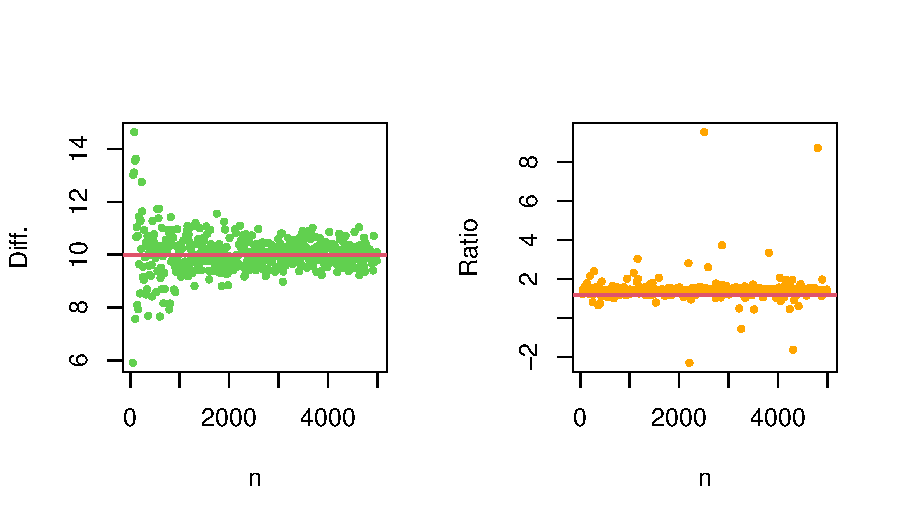
\includegraphics[width=\maxwidth]{figure/intro-lln4-0-1} 

}

\caption[Simulated test scores - difference and ratio between two groups]{Simulated test scores - difference and ratio between two groups.}\label{fig:intro-lln4-0}
\end{figure}

\begin{kframe}\begin{alltt}
\hlkwd{par}\hlstd{(}\hlkwc{mfrow}\hlstd{=}\hlkwd{c}\hlstd{(}\hlnum{1}\hlstd{,}\hlnum{1}\hlstd{))}
\end{alltt}
\end{kframe}
\end{knitrout}

What we see here is that the mean difference between the groups, $d_{AB}$, converges to the true difference between the groups (10), but the ratio, $r_{AB}$, does not converge -- $n$ can be as large as we want, and we will still see ratios that are quite extreme. (Note that the mean of a ratio between two distributions is generally not equal to the ratio of the means of the distributions, so we don't expect $r_{AB}$ to converge to exactly 70/60.)

What is happening here? The answer is that while a difference between two normal random variables is still normal (and hence, has a mean), the ratio between two normal distributions follows a Cauchy distribution which doesn't have a theoretical mean, so the LLN does not apply to  $r_{AB}$.

Although the LLN applies to almost any distribution we will ever encounter, the lesson here is that taking the ratio between two perfectly well-behaved distributions may lead to a distribution to which the LLN does not apply. Other manipulations of random variables may lead to similar results.



\section{The Central Limit Theorem}
The LLN says that as we increase the sample size, the sample mean converges to a fixed value (the true population mean).  It does not say anything, however, about how close the sample estimate is to the true value. In other words, it says nothing about our level of (un)certainty. 

The central limit theorem (CLT) says that, in many (most) situations, when independent random variables are averaged, their normalized mean tends toward a normal distribution. This is true even if the original variables themselves are not normally distributed!

To demonstrate it, we will use the previous examples.

